\documentclass[12pt]{article}
   
\usepackage[utf8]{inputenc}
   \usepackage{graphicx}
   \usepackage{float}
   \usepackage{subcaption}
   %\usepackage{mathtools}
   \usepackage{amsmath}
   \usepackage{listings}
    \usepackage{xcolor}
    
    \definecolor{codegreen}{rgb}{0,0.6,0}
    \definecolor{codegray}{rgb}{0.5,0.5,0.5}
    \definecolor{codepurple}{rgb}{0.58,0,0.82}
    \definecolor{backcolour}{rgb}{0.95,0.95,0.92}
    
    \lstdefinestyle{codestyle}{
        backgroundcolor=\color{backcolour},   
        commentstyle=\color{codegreen},
        keywordstyle=\color{magenta},
        numberstyle=\tiny\color{codegray},
        stringstyle=\color{codepurple},
        basicstyle=\ttfamily\footnotesize,
        breakatwhitespace=false,         
        breaklines=true,                 
        captionpos=b,                    
        keepspaces=true,                 
        numbers=left,                    
        numbersep=5pt,                  
        showspaces=false,                
        showstringspaces=false,
        showtabs=false,                  
        tabsize=2
    }
    
    \lstset{style=codestyle}

   \addtolength{\hoffset}{-0.7in}
   \addtolength{\textheight}{1.5in}
   \addtolength{\textwidth}{1.5in}
   \addtolength{\voffset}{-1in}
%
% Title.
\title{EE230: Experiment 4\\
Instrumentation Amplifier on load cell sensor}

% Author
\author{Hitesh Kandala, 180070023}

% begin the document.
\begin{document}

% make a title page.
\maketitle

\section{Overview of the experiment}

    \subsection{Aim of the experiment}
        \begin{itemize}
            \item In this experiment, we wish to implement instrumentation amplifier to amplify output from a load cell sensor. This is done in two parts:
            \begin{itemize}
                \item In part 1, we build the instrumentation amplifier using TL084 IC.
                \item In part 2, we implement the instrumentation amplifier using INA128 IC.
            \end{itemize}
            \item To observe/compare the output from the above two methods.
        \end{itemize}
        \begin{figure}[H]
            \centering
            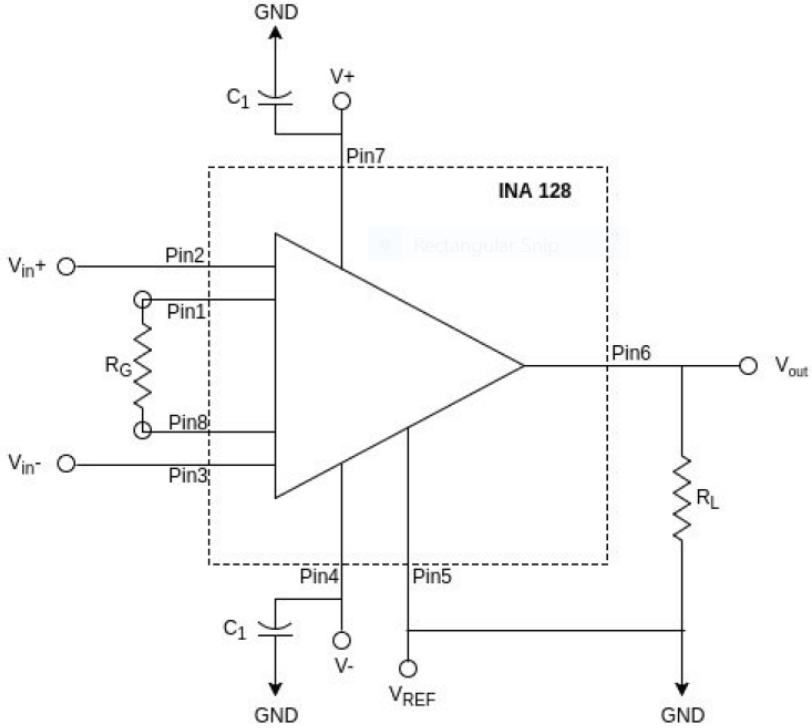
\includegraphics[width = 0.6\linewidth]{reports/lab4/INA.png}
            \caption{Pin diagram of INA128}
        \end{figure}

    \subsection{Theory}
        \subsubsection{Load Cell}
            A load cell is based on an electrical circuit called Wheatstone bridge. It consists of 4 strain gauges connected on a cantilever beam that undergo change in resistance when deformed (i.e. when the object to which they are connected to experiences strain).
            \begin{figure}[H]
                \centering
                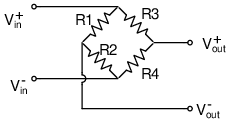
\includegraphics[width=0.5\linewidth]{reports/lab4/loadcell.png}
                \caption{Circuit Diagram of the Load Cell}
                \label{fig:loadcell}
            \end{figure}
            \\
            \noindent
            This arrangement allows to measure very small changes in the resistance R, which occurs in the strain gauges placed in the arms of the bridge: $R_1$, $R_2$, $R_3$ and $R_4$. When the load cell has no load, the four gauges are at rest and have the same ohmic value, the nominal value of the strain gauge Rg:
            \begin{equation}
                R_1 = R_2 = R_3 = R_4 = R_g 
            \end{equation}

            \begin{figure}[H]
              \centering
              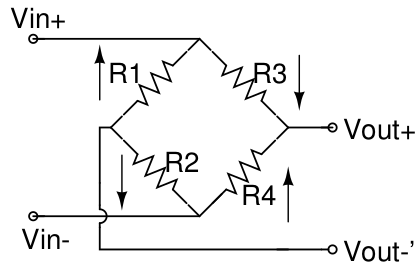
\includegraphics[width=0.5\linewidth]{reports/lab4/loadcell_strain.png}
              \caption{Strained resistors of Load Cell}
              \label{fig:instru}
            \end{figure}
            \noindent
            When the load cell experiences deformation due to externally applied force, the resistance of each strain gauge changes by a very small amount $\Delta R$. Hence, the differential voltage $\Delta V$ as a result of $\Delta R$ is as follows:
            \newpage
            % \begin{equation}
            %     R_1 = R_g + \Delta R; R_2 = R_g - \Delta R; R_3 = R_g - \Delta R; R_4 = R_g + \Delta R; 
            % \end{equation}
            % \noindent
            \begin{gather}
            	R1 = R_g + \Delta R \qquad R2 = R_g - \Delta R \qquad R3 = R_g - \Delta R \qquad R4 = R_g + \Delta R\\
            	\Delta V_{in} = V_{in}^+ - V_{in}^-\\
            	\text{As the resistors act as voltage dividers, we see}\\
            	V_{out}^+ = \frac{R_4}{R_4+R_3} \Delta V_{in}\\
            	V_{out}^- = \frac{R_2}{R_2+R_1} \Delta V_{in}\\
            	\Delta V_{out} = V_{out}^+ - V_{out}^-\\
            	\implies \Delta V_{out} = \left( \frac{R_g + \Delta R}{2R_g} - \frac{R_g - \Delta R}{2R_g} \right)\Delta V_{in}\\
            	\implies \Delta V_{out} = \frac{\Delta R}{R_g}\Delta V_{in}
            \end{gather}
            Hence we see that $V_{out}$ depends \textit{linearly} on $\Delta R$.
        
            \begin{figure}[H]
                \centering
                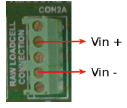
\includegraphics[width = 0.5\linewidth, height = 2.3in]{reports/lab4/5_connect.png}
                \caption{Raw load cell output to the input of instrumentation amplifier}
            \end{figure}
            
            \begin{figure}[H]
                \centering
                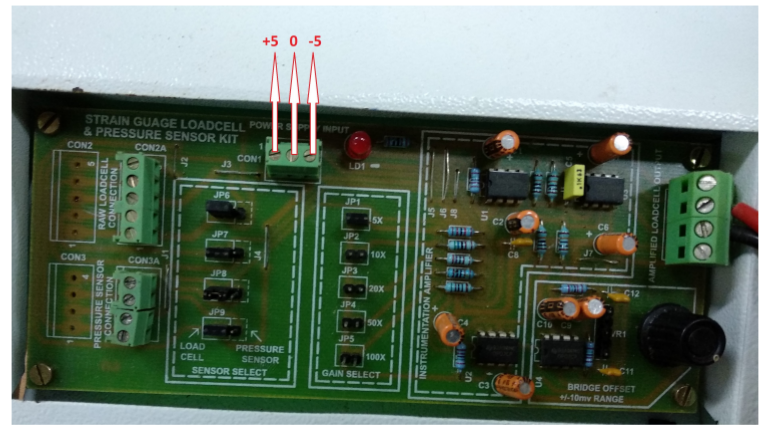
\includegraphics[width = 0.5\linewidth, height = 2.3in]{reports/lab4/5_power.png}
                \caption{Power supply connections to the weighing machine}
            \end{figure}
        \subsubsection{Instrumentation Amplifier}
            An instrumentation amplifier is a type of differential amplifier that has been outfitted with input buffer amplifiers. These input buffers eliminate the need for input impedance matching and thus make the amplifier particularly suitable for use in measurement and test equipment. Additional characteristics include very low DC offset, low drift, low noise, very high open-loop gain, very high common-mode rejection ratio, and very high input impedance. Instrumentation amplifiers are used to achieve high accuracy and stability.
            \\
            \begin{figure}[H]
              \centering
              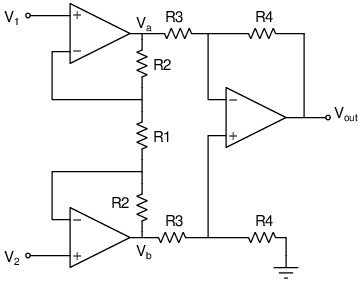
\includegraphics[width=0.8\linewidth]{reports/lab4/instrum.png}
              \caption{Circuit for Instrumentation Amplifier}
              \label{fig:instru}
            \end{figure}
            \noindent
            Here, we define the input voltage signals small signal AC differential input $V_1$ and $V_2$, as the input of first stage OPAMPs of the instrumentation amplifier. We assume input resistance of OPAMPs to be infinite. Now applying KCL at inverting input of first stage OPAMPs. We get,
            \begin{equation}
                V_a = V_1(1 + R_2/R_1) + V_2(R_2/R_1)
            \end{equation}
            \begin{equation}
                V_b = - V_1(R_2/R_1) + V_2(1 + R_2/R_1)
            \end{equation}
            Using superposition principle of voltages at second stage OPAMP,
            \begin{equation}
                V_{out} = R_4/R_3(1 + 2R_2/R_1)(V_2 - V_1)
            \end{equation}
            The gain is
            \begin{equation}
                A_v = \frac{V_{out}}{V_1 - V_2} = \frac{R_4}{R_3}(1 + \frac{2R_2}{R_1})
            \end{equation}
            
    
\newpage
\section{Experimental results}

    \subsection{Part 1 : Using Operational amplifier TL084}
        
        \textbf{Procedure}
        \begin{itemize}
            \item You will use Operational amplifier TL084. Refer to the data sheet of TL084.
            \item Refer to figure 6. Use Load Resistance of $10k\Omega$. $V_+=12V$, $V_-=-12V$ to
            power op-amp. Calculate the values of $R_1$, $R_2$, $R_3$ and $R_4$ properly to get a
            gain of about 300. Apply a single ended signal of $20mV_{p-p}$ 1kHz sine wave as input to tune the circuit to achieve the required amplification. Use decoupling capacitance if necessary.
            \item Connect power supply ($\pm5V$ and ground for bridge) to the weighing machine
            as shown in figure 5. Connect raw load cell output to the input
            of your 3 op-amp instrumentation amplifier. Refer to figure 4.
            \item Measure DMM voltage by varying weights. Calculate sensitivity of your
            instrumentation amplifier output to applied load in (mV/gm).
            \item Adjust $R_1$ value to double the sensitivity. Plot voltage vs weight to verify.
            \item Preserve the circuit of Part 1 till end of the experiment.
        \end{itemize}
        \noindent
        \textbf{Observations and Inferences}\\
        
        \noindent
        To get a gain of 300, we choose resistances $R_1$, $R_2$, $R_3$ and $R_4$ as $1k\Omega$, $1k\Omega$, $1k\Omega$ and $100k\Omega$.
        % \begin{equation}
        %     A_V & = \frac{R_4}{R_3}(1 + \frac{2R_2}{R_1})\\
        %         & = 100(1 + 2)\\
        %     A_V & = 300
        % \end{equation}
        \begin{align*} 
            A_V & = \frac{R_4}{R_3}(1 + \frac{2R_2}{R_1})\\
                & = 100(1 + 2)\\
                & = 300
        \end{align*}
        % \begin{figure}[H]
        %     \centering
        %     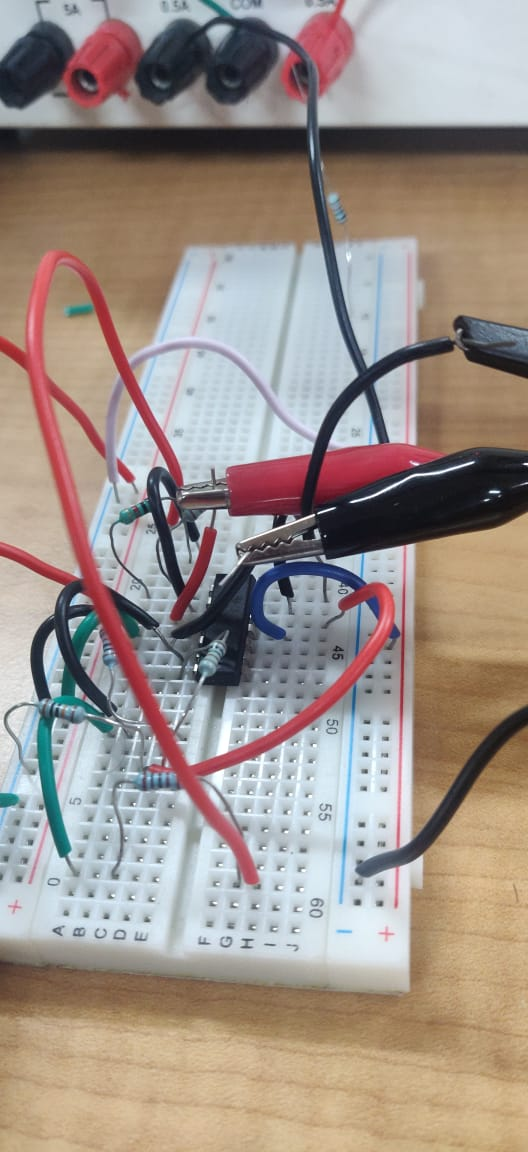
\includegraphics[width = 0.7\linewidth, height = 3.5in]{reports/lab4/circuit.jpeg}
        %     \caption{Physical circuit of Instrumentation amplifier}
        % \end{figure}
        \noindent
        The actual resistance values used in the figure 6 are $R_1 = 1k$, $R_2 = 1k$, $R_2 = 0.97k$, $R_3 = 0.98k$, $R_3 = 0.98k$, $R_4 = 98.9k$, $R_4 = 99.2k$
        \\\\
        $\ast$ Since the resistors value are not as desired there is some offset in the gains at the output of the first pair of op-amps which gets amplified from the last op-amp.
        \\\\
        \noindent
        $\ast$ The offset after the first pair of op-amps is -3.32mV and at the final output is 770mV.
        \\\\
        \noindent
        The waveforms of $V_{in}$ and $V_{out}$ can be seen in the figure below
        \begin{figure}[H]
            \centering
            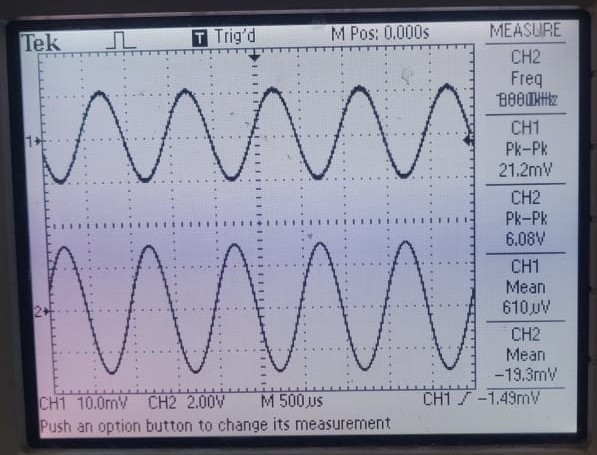
\includegraphics[width = 0.5\linewidth, height = 2.6in]{reports/lab4/amp.jpeg}
            \caption{Waveform of $V_{in}$ and $V_{out}$ for $A_V \approx 300$}
        \end{figure}
        \noindent
        Now using input from load cell sensor:
        \\
        We get the following results on the sensitivity of the instrumentation amplifier:
        
        \begin{figure}[H]
            \begin{subfigure}{0.7\linewidth}
                \centering
                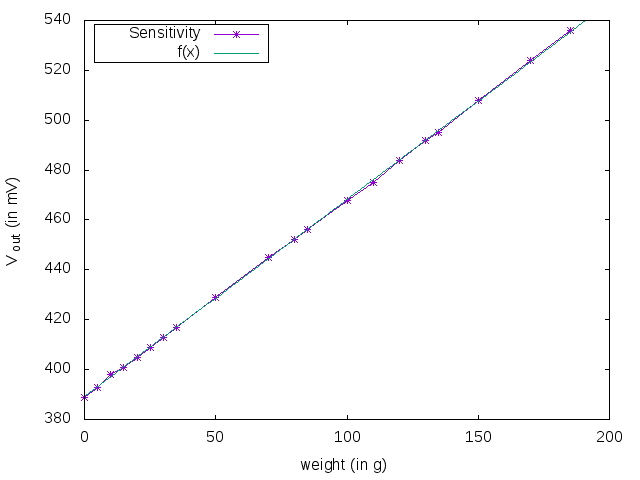
\includegraphics[width=\linewidth,height=4in]{reports/lab4/ownOp_1.png}
                \caption{Plot of output voltage vs weight for A_V \approx 300}
            \end{subfigure} 
            \begin{subfigure}{0.2\linewidth}
                \centering
                \begin{tabular}{|c|c|}
                \hline
                \bfseries $\mathbf{V_{out}(\text{in mV})}$	& \bfseries	$\mathbf{Weight(\text{in gm})}$	\\
                \hline
                    0  &		389 \\
                    5  &		393 \\
                    10 &    	398 \\
                    15 &		401 \\
                    20 &		405 \\
                    25 &		409 \\
                    30 &		413 \\
                    35 &		417 \\
                    50 &		429 \\
                    70 &		445 \\
                    80 &		452 \\
                    85 &		456 \\
                    100&		468 \\
                    110&		475 \\ 
                    120&		484 \\
                    130&		492 \\
                    135&		495 \\
                    150&		508 \\
                    170&		524 \\
                    185&		536 \\

                \hline
                \end{tabular}
            \end{subfigure} 
        \end{figure}
        \noindent
        The values of slope and intercept of the above plot are 0.789 and 389.22 respectively.
        \begin{equation}
            \boxed{\text{Sensitivity} = 0.79\; \text{mV/gm}} 
        \end{equation}
        \noindent
        Now we adjust $R_1$ value such that the gain gets double to approx 600.\\
        \noindent
        We can see this gain on the DSO in the figure below:
        
        \begin{figure}[H]
            \centering
            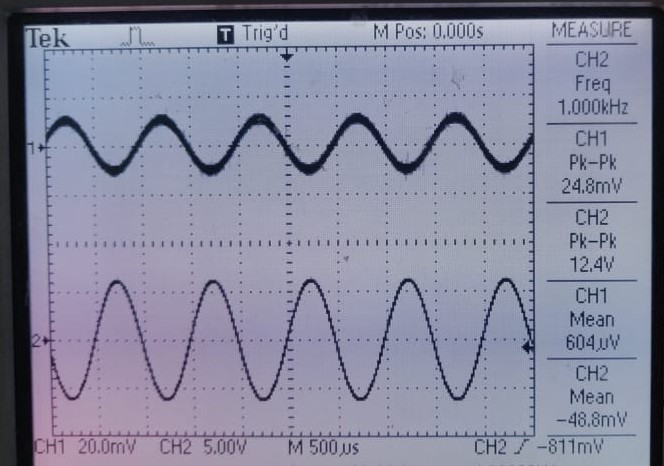
\includegraphics[width = 0.5\linewidth, height = 2.5in]{reports/lab4/ampli.jpeg}
            \caption{Waveform of $V_{in}$ and $V_{out}$ for $A_V \approx 600$}
        \end{figure}
        \noindent
        We get the following results on the sensitivity of the instrumentation amplifier for gain \approx 600:
        
        \begin{figure}[H]
            \begin{subfigure}{0.7\linewidth}
                \centering
                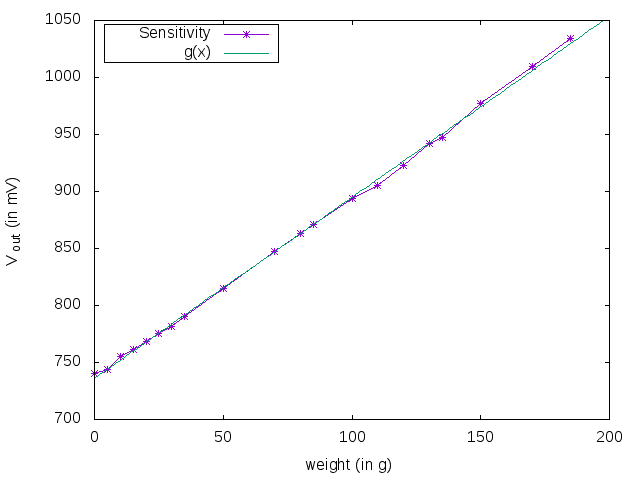
\includegraphics[width=\linewidth,height=4in]{reports/lab4/ownOp_2.png}
                \caption{Plot of output voltage vs weight for A_V \approx 600}
            \end{subfigure} 
            \begin{subfigure}{0.2\linewidth}
                \centering
                \begin{tabular}{|c|c|}
                \hline
                \bfseries $\mathbf{V_{out}(\text{in mV})}$	& \bfseries	$\mathbf{Weight(\text{in gm})}$	\\
                \hline
                    0	&				740 \\
                    5	&				744 \\
                    10	&				755 \\ 
                    15	&				761 \\
                    20	&				768 \\
                    25	&				775 \\ 
                    30	&				782 \\
                    35	&				790 \\
                    50	&				815 \\
                    70	&				847 \\
                    80	&				863 \\
                    85	&				871 \\
                    100	&				894 \\
                    110	&				905 \\
                    120	&				923 \\
                    130	&				942 \\
                    135	&				947 \\
                    150	&				977 \\ 
                    170	&				1010\\
                    185	&				1034\\
                \hline
                \end{tabular}
            \end{subfigure} 
        \end{figure}
        \noindent
        The values of slope and intercept of the above plot are 1.58 and 736.016 respectively.
        \begin{equation}
            \boxed{\text{Sensitivity} = 1.58\; \text{mV/gm}} 
        \end{equation}
        \noindent
        $\ast$ Therefore, as predicted the sensitivity got doubled.\\
        
        
    \subsection{Part 2 : Using Instrumentation Amplifier INA128}
    
        \textbf{Procedure}
        \begin{itemize}
            \item Now you will use instrumentation amplifier INA128 for load cell signal
            amplification. Refer to the data sheet of INA128.
            \item Using $R_G = 220\Omega$, $R_L = 10k\Omega$, $C_1 = 0.1\mu F$ , $V_+ = 12V$ , and $V_- = -12V$, wire up the instrumentation amplifier circuit. Refer to figure 1.
            Explain the purpose of capacitor $C_1$ connected in parallel with the power
            supply. Note polarity of $C_1$ and connect accordingly.
            \item Connect raw output (un-amplified differential output) of load cell to the
            designed instrumentation amplifier. Refer to figure 4.
            \item Note down the DMM voltage by varying weights. Plot voltage vs weight.
            Calculate sensitivity in (mV/gm).
            \item Adjust $R_G$ value such that you get twice the previous gain. Plot voltage vs weight.
        \end{itemize}
        
        \noindent
        \textbf{Observations and Inferences}
        \\\\
        \noindent
        $\ast$ The capacitor $C_1$ used in the above circuit is called the \textit{Decoupling Capacitor} which provides a low-resistance path for the noise/fluctuations that may occur in the power supply, which is a DC supply.
        \\\\
        Now using input from load cell sensor:
        \\\\
        Here, the gain depends on the external resistor $R_G$ as:
        
        \begin{equation}
            G = 1 + \frac{50k\Omega}{R_G}
        \end{equation}
        \noindent
        Therefore, for $R_G = 220\Omega$, $\mathbf{G = 228.27}$\\
        
        \begin{figure}[H]
          \centering
          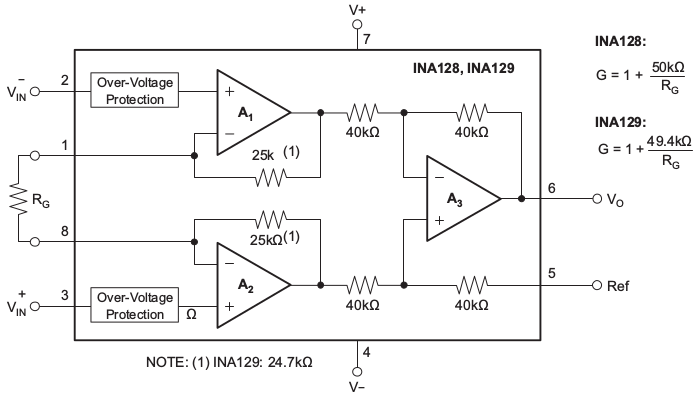
\includegraphics[width=0.7\linewidth]{reports/lab4/INA128.png}
          \caption{Schematic diagram of INA128}
          \label{fig:instru}
        \end{figure}
        \noindent
        We get the following results on the sensitivity of the instrumentation amplifier:
        \\\\
        \begin{figure}[H]
            \begin{subfigure}{0.7\linewidth}
                \centering
                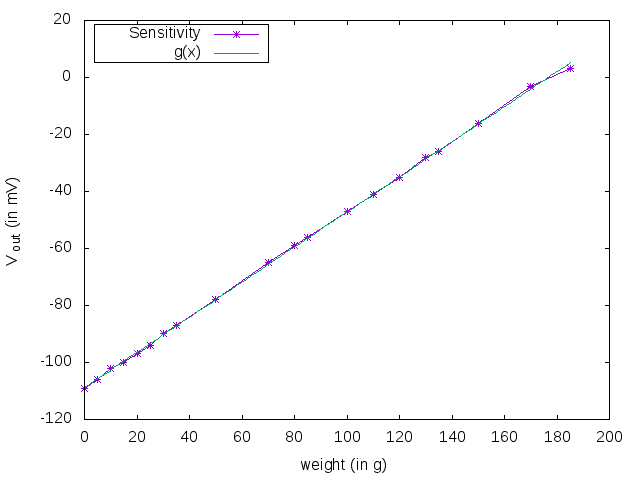
\includegraphics[width=\linewidth,height=4in]{reports/lab4/op_1.png}
                \caption{Plot of output voltage vs weight for G = 228.27}
            \end{subfigure} 
            \begin{subfigure}{0.2\linewidth}
                \centering
                \begin{tabular}{|c|c|}
                \hline
                \bfseries $\mathbf{V_{out}(\text{in mV})}$	& \bfseries	$\mathbf{Weight(\text{in gm})}$	\\
                \hline
                    0  &	-109 \\
                    5  &	-106 \\
                    10 &	-102 \\
                    15 &	-100 \\
                    20 &	-97  \\
                    25 &	-94  \\
                    30 &	-90  \\
                    35 &	-87  \\
                    50 &	-78  \\
                    70 &	-65  \\
                    80 &	-59  \\
                    85 &	-56  \\
                    100&	-47  \\
                    110&	-41  \\
                    120&	-35  \\
                    130&	-28  \\
                    135&	-26  \\
                    150&	-16  \\
                    170&	-3   \\
                    185&	3    \\

                \hline
                \end{tabular}
            \end{subfigure} 
        \end{figure}
        \noindent
        \\\\
        The values of slope and intercept of the above plot are 0.61 and -108.73 respectively.
        \\\\
        We could approximate gain as
        \\
        \begin{equation}
            G = 1 + \frac{50k\Omega}{R_G} \approx \frac{50k\Omega}{R_G}    
        \end{equation}
        \\
        \noindent
        since the resistor values that we are using are small. Therefore to double the gain, we connect another resistor of value $220\Omega$ in parallel with $R_G$.
        \begin{align*}
            R'_G & = R_G \, || \, 220\Omega\\
            R'_G & = 110\Omega 
        \end{align*}
        \noindent
        Therefore the gain for this new value of $R'_G$ is $\mathbf{G = 455.54}$ 
        \\\\
        \newpage
        \noindent
        We get the following results on the sensitivity of the instrumentation amplifier:
        
        \begin{figure}[H]
            \begin{subfigure}{0.7\linewidth}
                \centering
                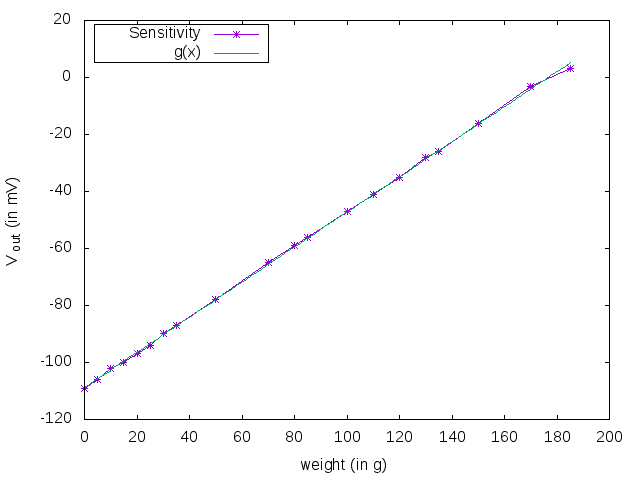
\includegraphics[width=\linewidth,height=5in]{reports/lab4/op_1.png}
                \caption{Plot of output voltage vs weight for G = 455.54}
            \end{subfigure} 
            \begin{subfigure}{0.2\linewidth}
                \centering
                \begin{tabular}{|c|c|}
                \hline
                \bfseries $\mathbf{V_{out}(\text{in mV})}$	& \bfseries	$\mathbf{Weight(\text{in gm})}$	\\
                \hline
                    0	&	-218	\\
                    5	&	-212	\\
                    10	&	-205	\\
                    15	&	-199	\\
                    20	&	-193	\\
                    25	&	-187	\\
                    30	&	-181	\\
                    35	&	-175	\\
                    50	&	-155	\\
                    70	&	-131	\\
                    80	&	-119	\\
                    85	&	-113	\\
                    100	&	-95	    \\
                    110	&	-82	    \\
                    120	&	-70	    \\
                    130	&	-58	    \\
                    135	&	-52	    \\
                    150	&	-33	    \\
                    170	&	-8	    \\
                    185	&	7	    \\

                \hline
                \end{tabular}
            \end{subfigure} 
        \end{figure}
        \noindent
        The values of slope and intercept of the above plot are 1.22 and -217.43 respectively.
        \\\\
        $\ast$ Here as well the slope got doubled for twice the gain.\\\\
        $\ast$ Another thing to note is that, the intercept which denotes the offset in the voltage at the output terminals of the op-amp also gets doubled indicating better impedance matching in the in-built instrumentation amplifier which was not the case in the instrumentation amplifier built by three op-amps in the first part.

\newpage
\section{Additional Questions}

    \textbf{(1)} Mention the reasons of the difference in performance of instrumentation
    amplifiers.\\
    \textbf{Ans:} The performance of the the instrumentation amplifier using INA128 should be better than that of using op-amp TL084, since there would be better matching of the resistors in the in-built IC thus reducing the noise and offset.
    \\\\
    \textbf{(2)} You measured the readings in parts 1, 2 and 3 with a DMM - observe the
    same on an oscilloscope. What do you observe? Is there a discrepancy?
    What is the reason for the discrepancy, if any?\\
    \textbf{Ans:} On oscilloscope, we see that the waveform is somewhat periodic and quite noisy.
    \begin{figure}[H]
        \centering
        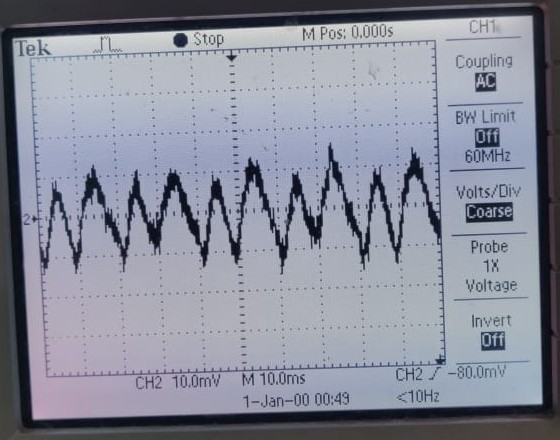
\includegraphics[width = 0.5\linewidth, height = 2.6in]{reports/lab4/extra2.jpeg}
        \caption{Waveform of part 2 as seen in DSO}
    \end{figure}
    \noindent
    The oscilloscope picks up noise from the surroundings as is seen in the below figure.
    \begin{figure}[H]
        \centering
        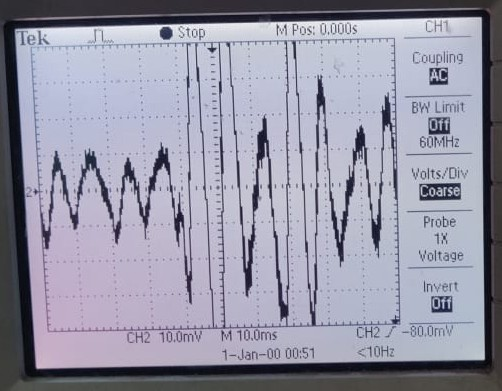
\includegraphics[width = 0.5\linewidth, height = 2.6in]{reports/lab4/extra.jpeg}
        \caption{Above waveform with noise indicating high sensitivity to surroundings}
    \end{figure}
\section{Pre-Lab}
    Here is the code used in simulating the instrumentation amplifier we implemented using TL084 :
    \begin{lstlisting}
Instrumentation Amplifier Using the IC TL084
.include TL084_model_file.txt
x1 11 1 12 13 3 TL084
x2 10 9 12 13 8 TL084
x3 4 7 12 13 6 TL084
r1 9 1 1k
r2 3 1 1k
r3 8 9 1k
r4 3 4 1k
r5 8 7 1k
r6 7 6 10k
r7 4 0 100k
r8 6 0 100k
vcc 12 0 dc 15v
vee 13 0 dc -15v
vin1 11 0 sin (0 20mV 1k 0 0)
vin2 10 0 sin (0 0mV 1k 0 0)
.tran .1ms 10ms
.control
run
plot V(6) (V(11)-V(10))
.endc
.end
\end{lstlisting}
    Its simulation output can be seen in the figure below.
    \begin{figure}[H]
      \centering
      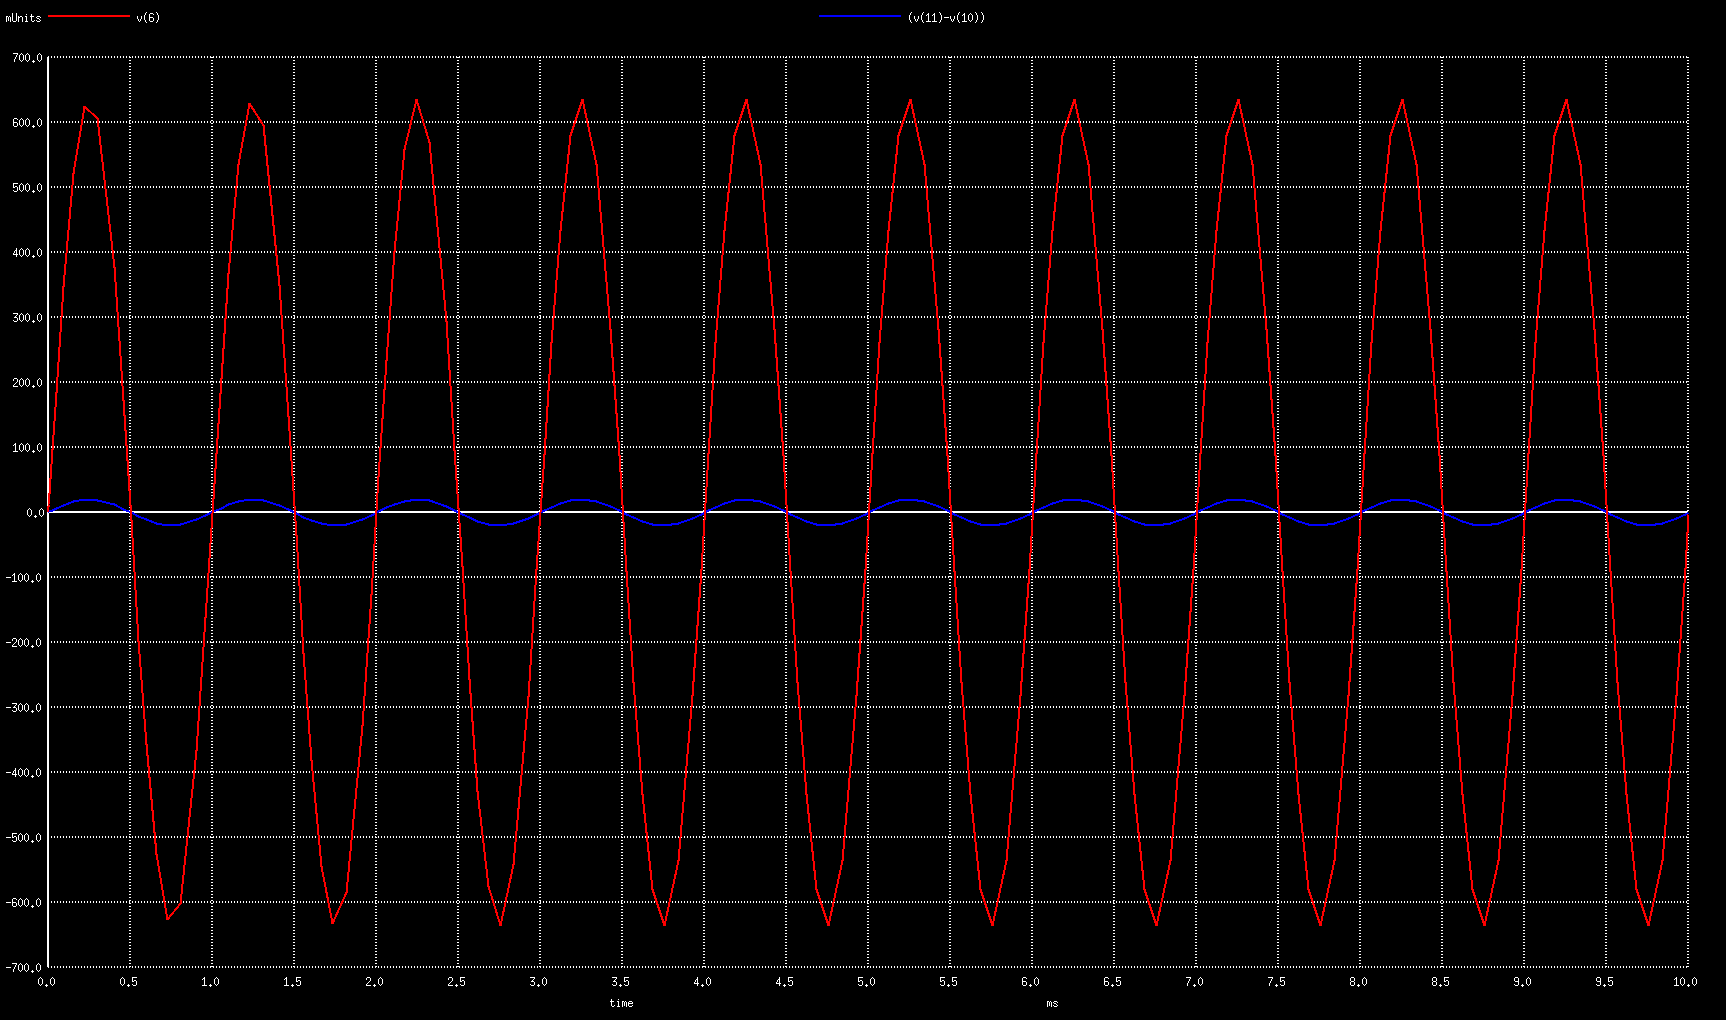
\includegraphics[width=0.8\linewidth]{reports/lab4/5_spice.png}
      \caption{Plot of $\Delta V_{out}$ vs $\Delta V_{in}$, $A_v = 300$}
    \end{figure}
\noindent
The TL084$\_$model$\_$file.txt file has the following code:
\begin{lstlisting}
* TL084 OPERATIONAL AMPLIFIER "MACROMODEL" SUBCIRCUIT
* CREATED USING PARTS RELEASE 4.01 ON 06/16/89 AT 13:08
* (REV N/A)      SUPPLY VOLTAGE: +/-15V
* CONNECTIONS:   NON-INVERTING INPUT
*                | INVERTING INPUT
*                | | POSITIVE POWER SUPPLY
*                | | | NEGATIVE POWER SUPPLY
*                | | | | OUTPUT
*                | | | | |
.SUBCKT TL084    1 2 3 4 5
*
  C1   11 12 3.498E-12
  C2    6  7 15.00E-12
  DC    5 53 DX
  DE   54  5 DX
  DLP  90 91 DX
  DLN  92 90 DX
  DP    4  3 DX
  EGND 99  0 POLY(2) (3,0) (4,0) 0 .5 .5
  FB    7 99 POLY(5) VB VC VE VLP VLN 0 4.715E6 -5E6 5E6 5E6 -5E6
  GA    6  0 11 12 282.8E-6
  GCM   0  6 10 99 8.942E-9
  ISS   3 10 DC 195.0E-6
  HLIM 90  0 VLIM 1K
  J1   11  2 10 JX
  J2   12  1 10 JX
  R2    6  9 100.0E3
  RD1   4 11 3.536E3
  RD2   4 12 3.536E3
  RO1   8  5 150
  RO2   7 99 150
  RP    3  4 2.143E3
  RSS  10 99 1.026E6
  VB    9  0 DC 0
  VC    3 53 DC 2.200
  VE   54  4 DC 2.200
  VLIM  7  8 DC 0
  VLP  91  0 DC 25
  VLN   0 92 DC 25
.MODEL DX D(IS=800.0E-18)
.MODEL JX PJF(IS=15.00E-12 BETA=270.1E-6 VTO=-1)
.ENDS

\end{lstlisting}

\section{In Lab Circuit}
    \begin{figure}[H]
      \centering
      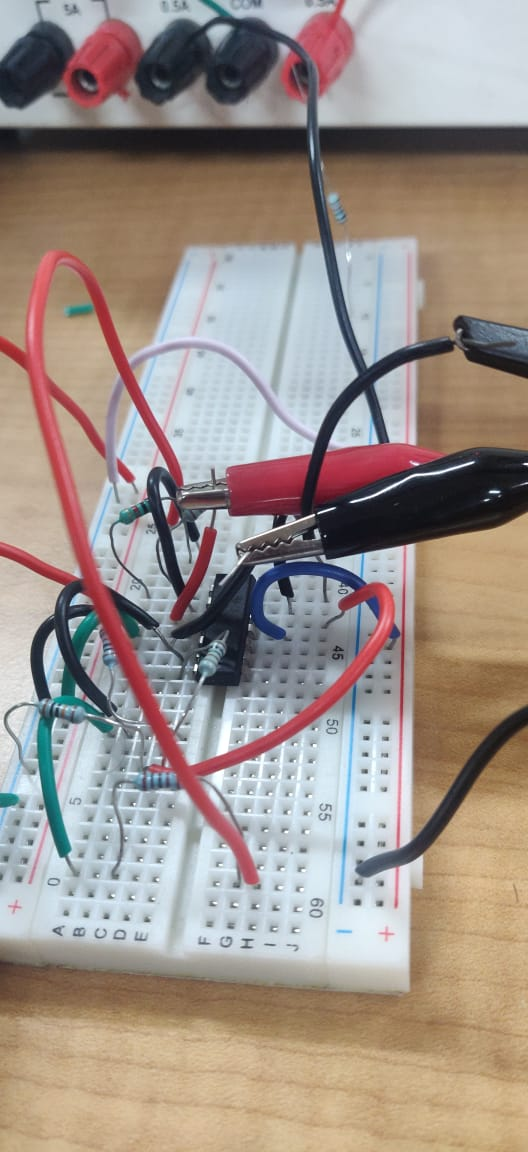
\includegraphics[width=0.5\linewidth]{reports/lab4/circuit.jpeg}
      \caption{Circuit of instrumentation amplifier on breadboard}
      \label{fig:instru}
    \end{figure}
    
    \begin{figure}[H]
      \centering
      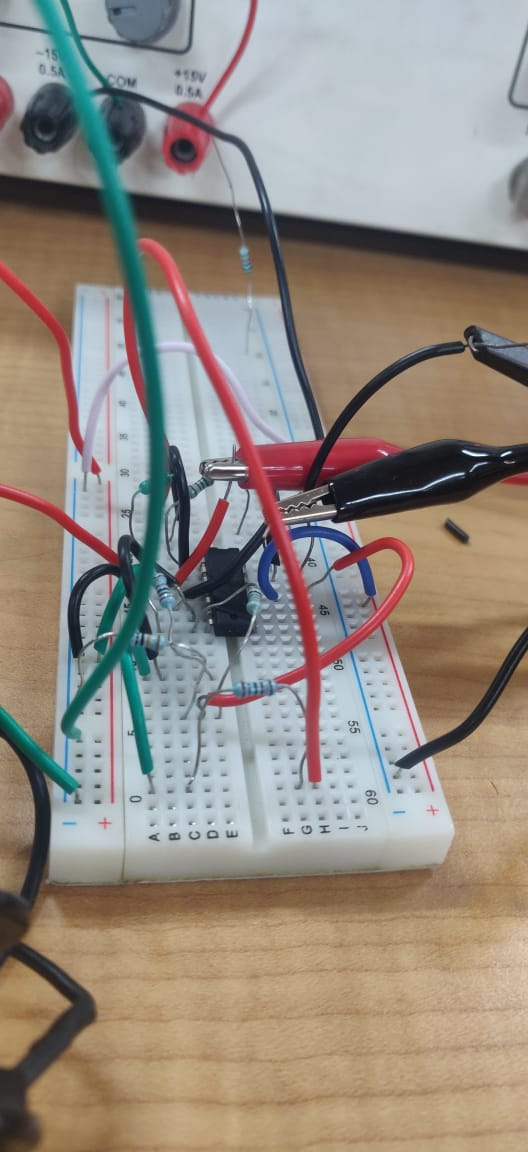
\includegraphics[width=0.5\linewidth]{reports/lab4/circuit2.jpeg}
      \caption{Circuit of instrumentation amplifier on breadboard}
      \label{fig:instru}
    \end{figure}
      
\vspace{4cm}

    \begin{thebibliography}{9}

        \bibitem{Analog LAB Manual} 
        Experiment Handout 
        \\\texttt{http://wel.ee.iitb.ac.in/teaching\_labs/WEL\%20Site/ee230/Labsheets\-2020/Handouts/Instrumentation\%20\_amp\_LoadCell.pdf}
        \bibitem{Datasheet of UA741}
        Supporting material for Instrumentation amplifier with datasheet of TL084 and INA128
        \\\texttt{http://wel.ee.iitb.ac.in/teaching\_labs/WEL\%20Site/ee230/Labsheets\-2020/supporting\_documents/Instrumentation\_loadcell.zip}
        
    \end{thebibliography}

\end{document}

